\documentclass[11pt]{article}
\usepackage[utf8]{inputenc}
\usepackage{fancyhdr}
\usepackage{natbib}
\usepackage{amsfonts, amsmath, amsthm, amssymb}
\usepackage{lipsum}
\usepackage[legalpaper, portrait, margin=1.2in]{geometry}
\usepackage[parfill]{parskip}
\usepackage[autostyle]{csquotes}
\usepackage[shortlabels]{enumitem}
\usepackage{verbatim}
\usepackage{graphicx}
\usepackage[]{physics}
\usepackage[]{float}
\usepackage[]{breqn}
\usepackage{ dsfont }
\usepackage{xcolor}
\usepackage{listings}

\usepackage[]{natbib}
\usepackage{hyperref}
\hypersetup{
    colorlinks=true,
    linkcolor=blue,
    filecolor=magenta,      
    urlcolor=blue,
    pdftitle={Overleaf Example},
    pdfpagemode=FullScreen,
    citecolor=blue
    }
\urlstyle{same}


\usepackage[]{tikz}
\usetikzlibrary{arrows.meta}

\pagestyle{fancy}
\fancyhead{}
\fancyfoot{}
\fancyhead[L]{\slshape \MakeUppercase{Quantum Algorithms}}
\fancyhead[R]{\slshape Yangda Bei}
\fancyfoot[CO,C]{\thepage}
\fancyfoot[RO,R]{}

\renewcommand{\headrulewidth}{0.4pt}
\renewcommand{\footrulewidth}{0.4pt}

\newenvironment{theorem}[2][Theorem]{\begin{trivlist}
\item[\hskip \labelsep {\bfseries #1}\hskip \labelsep {\bfseries #2.}]}{\end{trivlist}}
\newenvironment{lemma}[2][Lemma]{\begin{trivlist}
\item[\hskip \labelsep {\bfseries #1}\hskip \labelsep {\bfseries #2.}]}{\end{trivlist}}
\newenvironment{exercise}[2][Exercise]{\begin{trivlist}
\item[\hskip \labelsep {\bfseries #1}\hskip \labelsep {\bfseries #2.}]}{\end{trivlist}}
\newenvironment{problem}[2][Problem]{\begin{trivlist}
\item[\hskip \labelsep {\bfseries #1}\hskip \labelsep {\bfseries #2.}]}{\end{trivlist}}
\newenvironment{question}[2][Question]{\begin{trivlist}
\item[\hskip \labelsep {\bfseries #1}\hskip \labelsep {\bfseries #2.}]}{\end{trivlist}}
\newenvironment{corollary}[2][Corollary]{\begin{trivlist}
\item[\hskip \labelsep {\bfseries #1}\hskip \labelsep {\bfseries #2.}]}{\end{trivlist}}

\newenvironment{solution}{\begin{proof}[Solution]}{\end{proof}}
\newcommand{\lr}[3]{\!\left#1 #3 \right#2}

\newcommand{\p}{\varphi}
\newcommand{\s}{\sigma}
\newcommand{\R}{\mathbb{R}}

\title{QAOA on MaxCut Practice Problems}


\begin{document}
    \maketitle


    \begin{question}{1}
        Consider the following graph:
        \begin{figure}[H]
        \begin{center}
            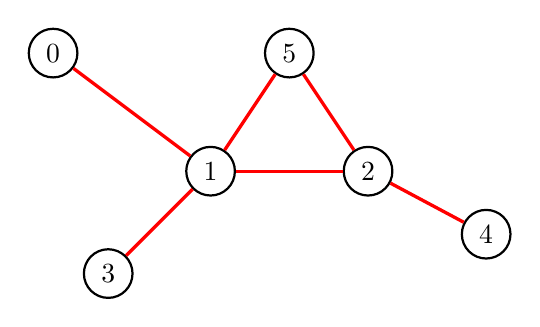
\begin{tikzpicture}
                \begin{scope}[every node/.style={circle,thick,draw}]
                    \node (1) at (-3,1.5) {0};
                    \node (2) at (-1,0) {1};
                    \node (3) at (1,0) {2};
                    \node (4) at (-2.3,-1.3) {3};
                    \node (5) at (2.5,-0.8) {4};
                    \node (6) at (0,1.5) {5} ;
                \end{scope}
                \begin{scope}[>={Stealth[black]},
                    every node/.style={fill=white,circle},
                    every edge/.style={draw=red,very thick}]
                    \path [-] (1) edge (2);
                    \path [-] (4) edge (2);
                    \path [-] (6) edge (2);
                    \path [-] (6) edge (3);
                    \path [-] (2) edge (3);
                    \path [-] (3) edge (5);
                \end{scope}
            \end{tikzpicture}
        \end{center}
        \caption{Graph 1}
        \end{figure}
        
        \begin{enumerate}[(a)]
            \item 
            Find the exact max-cut for this graph.
            \begin{solution}
                The exact max-cut for this graph is 5.
            \end{solution}
            \item
            The Goemans-Williamson algorithm gives an approximate solution to the max-cut problem with an approximation ratio of at lease 0.868. Use the Goemans-Williamson algorithm to find an approximate solution to this graph.
            \begin{solution}
                The following code from \href{https://www.youtube.com/watch?v=aFVnWq3RHYU}{this video} was implemented. 

                \begin{figure}[H]
                    \centering
                    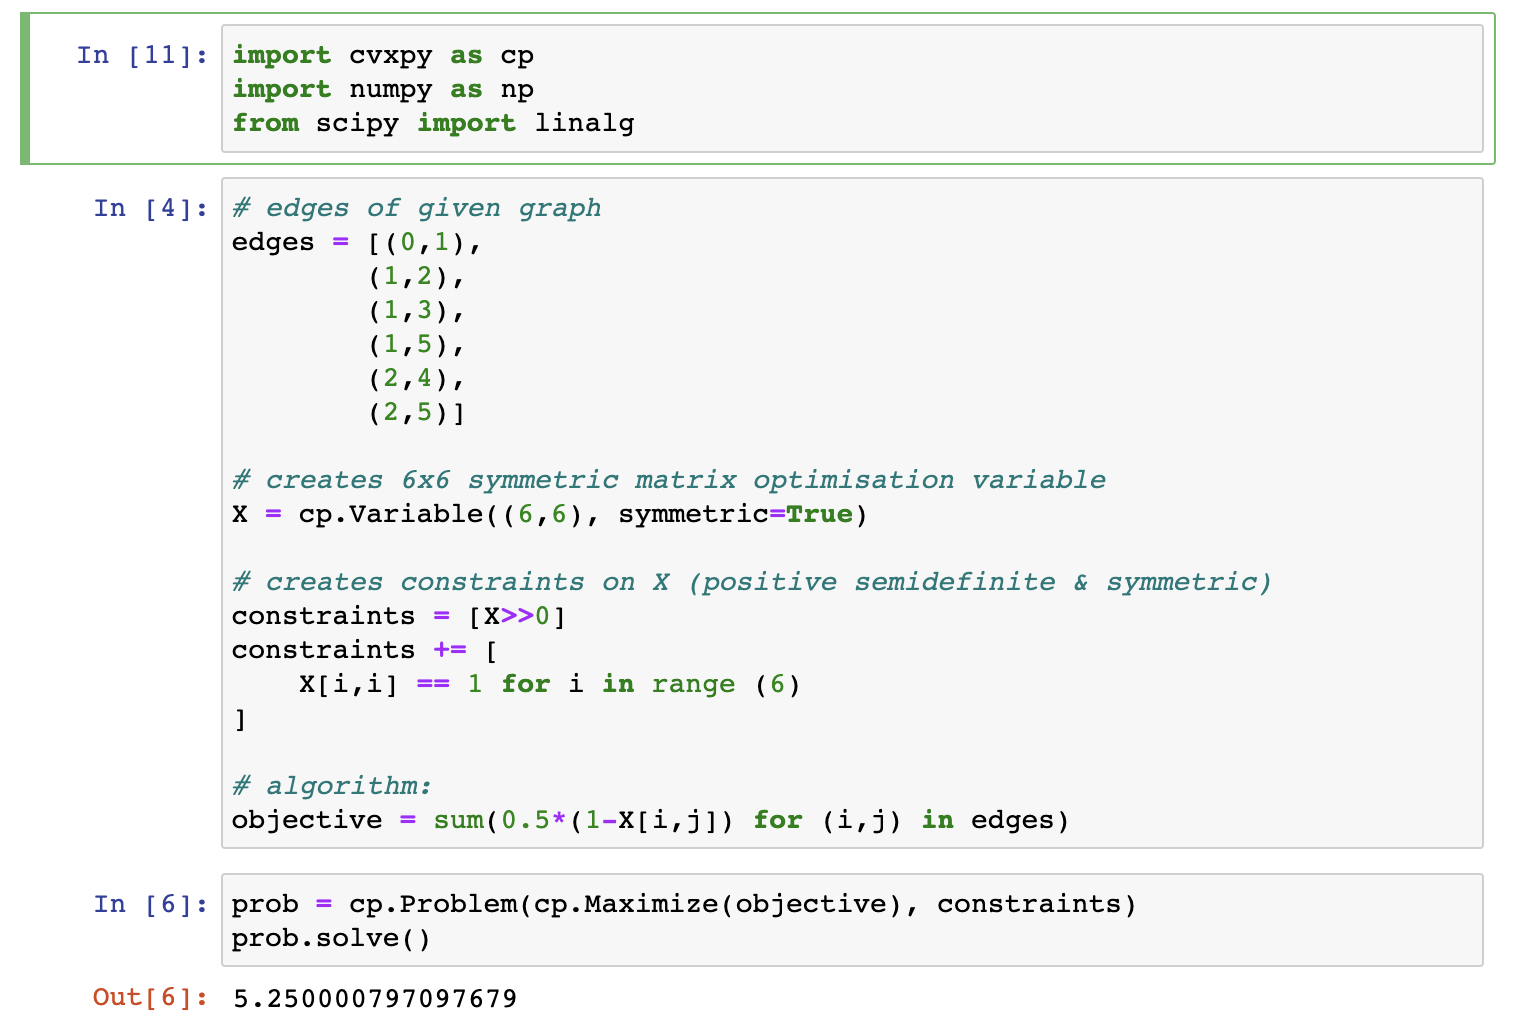
\includegraphics[scale=0.5]{Screen Shot 2022-12-19 at 22.59.27.png}
                \end{figure}

                \begin{lstlisting}[language=Python, caption=Python example]
    import cvxpy as cp
    from scipy import linalg

    # edges of given graph
    edges = [(0,1), (1,2), (1,3), (1,5), (2,4), (2,5)]
    # creates 6x6 symmetric matrix optimisation variable
    X = cp.Variable((6,6), symmetric=True)
    # creates constraints on X (positive semidefinite 
    # & symmetric)
    constraints = [X>>0]
    constraints += [X[i,i] == 1 for i in range (6)]
    
    # algorithm: 
    objective = sum(0.5*(1-X[i,j]) for (i,j) in edges)
                \end{lstlisting}

                The cost was found to be 5.25, yielding a max-cut of 5 for the graph.  
            \end{solution}
        \end{enumerate}
    \end{question}

    \begin{question}{2}
        Our goal is to derive an analytic expression for the expectation value for $p=1$ in the Max-Cut problem. Consider the state
        $$|\gamma,\beta\rangle = U_B(\beta)U_C(\gamma)|s\rangle,$$
        where $|s\rangle=|+,+,\dots,+\rangle$ is the state where all qubits are initialised to the plus state and $U_B(\beta)=e^{-i\beta B}$ and $U_C(\gamma)=e^{-i\gamma C}$. For an edge $(u,v)$, we want to derive ana analytic expression for $\langle\gamma,\beta|C_{uv}|\gamma,\beta\rangle$, where $C_{uv}=\frac{1}{2}(1-Z_uZ_v)$.
        \begin{enumerate}[(a)]
            \item 
            Show that:
            $$e^{i\beta X_u}Z_ue^{-i\beta X_u}=e^{2i\beta X_u}Z_u.$$
            \begin{solution}
                For matrices $A,B,C,D$, the mixed-product property of the tensor product states that
                $$(A\otimes B)(C\otimes D) = (AC)\otimes(BD).$$
                $X_u$ and $Z_u$ are tensor products of the identity and $\sigma_x$ and $\sigma_z$ respectively where $\sigma_x$ and $\sigma_z$ are in the $u^{th}$ position of the product. This means that the $\sigma_{i_u}$ follows the commutator relationships. We get that
                \begin{align*}
                    e^{i(\beta) X_u}Z_ue^{-i(\beta) X_u} &= \lr(){\cos(\beta)+iX_u\sin(\beta)}Z_u\lr(){\cos(\beta)-iX_u\sin(\beta)} \\
                    &= \lr(){\cos(\beta)+iX_u\sin(\beta)}\lr(){Z_u\cos(\beta)-iZ_uX_u\sin(\beta)} \\
                    &= \cos^2(\beta) Z_u-i\cos\beta\sin(\beta) Z_uX_u + i\cos(\beta)\sin(\beta) X_uZ_u  \\
                    &\quad \quad \quad \quad + \sin^2(\beta) X_uZ_uX_u \\
                    &= \cos^2(\beta) Z_u +\cos(\beta)\sin(\beta) Y_u + \cos(\beta)\sin(\beta) Y_u-\sin^2(\beta) Z_u \\
                    &= \lr(){\cos^2(\beta) -\sin^2(\beta)} Z_u + \sin(2\beta) Y_u \\
                    &= \cos(2\beta)Z_u+\sin(2\beta)Y_u \\
                    &= \cos(2\beta)Z_u +i\sin(2\beta)X_uZ_u \\
                    &= \lr(){\cos{2\beta}+iX_u\sin(2\beta)}Z_u \\
                    &= e^{2i\beta X_u}
                \end{align*}
            \end{solution}

            \item
            Show that:
            \begin{align*}
                e^{i\beta B}Z_uZ_ve^{-i\beta B} &= e^{2i\beta X_u}Z_ue^{2i\beta X_v}Z_v \\
                &= \cos^2(2\beta)Z_uZ_v+\cos(2\beta)\sin(2\beta)(Z_uY_v+Y_uZ_v)+\sin^2(2\beta)Y_uY_v
            \end{align*}
            \begin{solution}
                First, consider $Z_1$ and $Z_2$ acting on two qubits. Then 
                \begin{align*}
                    (Z_1\otimes\mathds{1})(\mathds{1}\otimes Z_2) &= Z_1\mathds{1} \otimes \mathds{1}Z_2 \\
                    &= \mathds{1}Z_1 \otimes Z_2\mathds{1} \\
                    &= (\mathds{1}\otimes Z_2) (Z_1\otimes\mathds{1}).
                \end{align*}
                This means that $Z_i$ commutes with $Z_j$ for $i\neq j$. Fix two nodes, $u$ and $v$. We get that
                \begin{align*}
                    e^{i\beta B}Z_uZ_ve^{-i\beta B} &= \prod_ne^{i\beta X_n}Z_uZ_v\prod_m e^{-i\beta X_m} \\
                    &= e^{i\beta X_u}Z_ue^{-i\beta X_u}e^{i\beta X_v}Z_ve^{-i\beta X_v} \\
                    &= e^{2i\beta X_u}Z_ue^{2i\beta X_v}Z_v.
                \end{align*}
                For the second part, we get
                \begin{align*}
                    e^{2i\beta X_u}Z_ue^{2i\beta X_v}Z_v &= \lr(){\cos(2\beta)+iX_u\sin(2\beta)}Z_u\lr(){\cos(2\beta)+iX_v\sin(2\beta)}Z_v \\
                    &= \lr(){\cos(2\beta)+iX_u\sin(2\beta)}Z_u\lr(){\cos(2\beta)Z_v+i\sin(2\beta)X_vZ_v} \\
                    &= \lr(){\cos(2\beta)+iX_u\sin(2\beta)}\lr(){\cos(2\beta)Z_uZ_v+i\sin(2\beta)Z_uX_vZ_v} \\
                    &= \lr(){\cos(2\beta)+iX_u\sin(2\beta)}\lr(){\cos(2\beta)Z_uZ_v+\sin(2\beta)Z_uY_v} \\ 
                    &= \cos^2(2\beta)Z_uZ_v+\cos(2\beta)\sin(2\beta)Z_uY_v \\
                    &\quad\quad\quad +i\sin(2\beta)\cos(2\beta)X_uZ_uZ_v+i\sin^2(2\beta)X_uZ_uY_v \\
                    &= \cos^2(2\beta)Z_uZ_v+\cos(2\beta)\sin(2\beta)Z_uY_v \\
                    &\quad\quad\quad+\sin(2\beta)\cos(2\beta)Y_uZ_v+\sin^2(2\beta)Y_uY_v \\
                    &= \cos^2(2\beta)Z_uZ_v+\cos(2\beta)\sin(2\beta)(Z_uY_v+Y_uZ_v)+\sin^2(2\beta)Y_uY_v.
                \end{align*}
            \end{solution}

            \item
            To evaluate $\left\langle\gamma, \beta\left|C_{u v}\right| \gamma, \beta\right\rangle$, we need to evaluate the four terms $\left\langle s\left|e^{i \gamma C} Z_u Z_v e^{-i \gamma C}\right| s\right\rangle$, $\left\langle s\left|e^{i \gamma C} Z_u Y_v e^{-i \gamma C}\right| s\right\rangle$, $\left\langle s\left|e^{i \gamma C} Y_u Z_v e^{-i \gamma C}\right| s\right\rangle$ and $\left\langle s\left|e^{i \gamma C} Y_u Y_v e^{-i \gamma C}\right| s\right\rangle$.

            Show that:
            \begin{itemize}
                \item $\left\langle s\left|e^{i \gamma C} Z_u Z_v e^{-i \gamma C}\right| s\right\rangle=0$
                \item $\left\langle s\left|e^{i \gamma C} Z_u Y_v e^{-i \gamma C}\right| s\right\rangle=-\sin \gamma \cos ^e \gamma$
                \item $\left\langle s\left|e^{i \gamma C} Y_u Z_v e^{-i \gamma C}\right| s\right\rangle=-\sin \gamma \cos ^d \gamma$
                \item $\left\langle s\left|e^{i \gamma C} Y_u Y_v e^{-i \gamma C}\right| s\right\rangle=(\cos \gamma)^{d+e-2 f}\left(1-\cos ^f 2 \gamma\right) / 2$,
              \end{itemize}
            where $d$ and $e$ are the number of neighbours for nodes $u$ and $v$ minus 1. $f$ is the number of triangles (nodes that are connected to both $u$ and $v$).
            \begin{solution}
                Fix two nodes, $u$ and $v$. To show the first equation, we start with 
                \begin{align*}
                    \left\langle s\left|e^{i \gamma C} Z_u Z_v e^{-i \gamma C}\right| s\right\rangle &= \left\langle s\left|\prod_\alpha e^{i\gamma C_\alpha}Z_uZ_v \prod_\alpha e^{-i\gamma C_\alpha}\right|s\right\rangle \\
                    &= \left\langle s\left|\prod_{\langle jk\rangle} e^{i\gamma C_{\langle jk\rangle} }Z_uZ_v \prod_{\langle jk\rangle} e^{-i\gamma C_{\langle jk\rangle}}\right|s\right\rangle \\
                    &= \left\langle s\left|\prod_{\langle jk\rangle} e^{\frac{i\gamma}{2}(1-Z_jZ_k) }Z_uZ_v \prod_{\langle jk\rangle} e^{-\frac{i\gamma}{2}(1-Z_jZ_k)}\right|s\right\rangle \\
                    &= \left\langle s\left|\prod_{\langle jk\rangle} e^{\frac{i\gamma}{2}}e^{-\frac{i\gamma}{2}Z_jZ_k }Z_uZ_v \prod_{\langle jk\rangle} e^{-\frac{i\gamma}{2}}e^{\frac{i\gamma}{2}Z_jZ_k }\right|s\right\rangle 
                \end{align*}
                Since the expectation value remains invariant under a global phase shift, we can remove all factors of $e^{\frac{i\gamma}{2}}$ and $e^{-\frac{i\gamma}{2}}$. Next, since any terms not involving $u$ or $v$ commute with $Z_u$ and $Z_v$, we can move them around so that they cancel with their conjugates. We then get that
                \begin{align*}
                    &= \left\langle s\left|e^{-\frac{i\gamma}{2}Z_uZ_v }Z_uZ_v e^{\frac{i\gamma}{2}Z_uZ_v }\right|s\right\rangle \\
                    &= \left\langle s\left|\lr(){\cos\lr(){\frac{\gamma}{2}}-i\sin\lr(){\frac{\gamma}{2}}Z_uZ_v}Z_uZ_v \lr(){\cos\lr(){\frac{\gamma}{2}}+i\sin\lr(){\frac{\gamma}{2}}Z_uZ_v}\right|s\right\rangle \\
                    &= \left\langle s\left|\lr(){\cos\lr(){\frac{\gamma}{2}}-i\sin\lr(){\frac{\gamma}{2}}Z_uZ_v} \lr(){\cos\lr(){\frac{\gamma}{2}}Z_uZ_v+i\sin\lr(){\frac{\gamma}{2}}(Z_uZ_v)^2}\right|s\right\rangle \\
                    &= \lr\langle\rangle{s\lr||{\lr[]{\cos^2\lr(){\frac{\gamma}{2}}+i\sin\lr(){\frac{\gamma}{2}}\cos\lr(){\frac{\gamma}{2}}Z_uZ_v - i\sin\lr(){\frac{\gamma}{2}}\cos\lr(){\frac{\gamma}{2}}Z_uZ_v + \sin^2\lr(){\frac{\gamma}{2}}(Z_uZ_v)^2}Z_uZ_v}s} \\
                \end{align*}
                Since $Z_u$ and $Z_v$ commute, $(Z_uZ_v)^2 = Z_u^2Z_v^2=1$. We get that
                \begin{align*}
                    \langle s|Z_uZ_v|s\rangle = 0
                \end{align*}
                since $Z$ gates collapses $|+\rangle$.

                For the second equation, we get 
                \begin{align*}
                    \left\langle s\left|e^{i \gamma C} Z_u Y_v e^{-i \gamma C}\right| s\right\rangle &= \left\langle s\left|\prod_{\langle jk\rangle} e^{\frac{i\gamma}{2}}e^{-\frac{i\gamma}{2}Z_jZ_k }Z_uY_v \prod_{\langle jk\rangle} e^{-\frac{i\gamma}{2}}e^{\frac{i\gamma}{2}Z_jZ_k }\right|s\right\rangle 
                \end{align*}
                Again, we can ignore the global phase shift. Then
                \begin{align*}
                    &= \left\langle s\left|\prod_{\langle jk\rangle} e^{-\frac{i\gamma}{2}Z_jZ_k }Z_uY_v \prod_{\langle jk\rangle} e^{\frac{i\gamma}{2}Z_jZ_k }\right|s\right\rangle 
                \end{align*}
                Now, note that $Y_v$ anticommutes with any term containing $Z_v$ in the product on the right. Elements containin $Z_v$ are nodes in the neighbourhood of $v$, denoted $N(v)$. Consider a product $Y_v(\cos\frac{\gamma}{2}+i\sin\frac{\gamma}{2}Z_vZ_w)$ for some $w$. We have that $Y_v(\cos\frac{\gamma}{2}+i\sin\frac{\gamma}{2}Z_vZ_w)=(\cos\frac{\gamma}{2}Y_v+i\sin\frac{\gamma}{2}y_vZ_vZ_w)=(\cos\frac{\gamma}{2}Y_v-i\sin\frac{\gamma}{2}Z_vY_vZ_w)=(\cos\frac{\gamma}{2}-i\sin\frac{\gamma}{2}Z_vZ_w)Y_v$. Continuing our derivation gives
                \begin{align*}
                    &= \lr\langle\rangle{s\lr||{\prod_{\langle jk\rangle}e^{-\frac{i\gamma}{2}Z_jZ_k}\prod_{\langle jk\rangle \setminus N(v)}e^{\frac{i\gamma}{2}Z_jZ_k}\prod_{w\in N(v)}e^{-\frac{i\gamma}{2}Z_wZ_v}Z_uY_v}s} \\
                    &= \lr\langle\rangle{s\lr||{\prod_{w\in N(v)}e^{-\frac{i\gamma}{2}Z_wZ_v}\prod_{w\in N(v)}e^{-\frac{i\gamma}{2}Z_wZ_v}Z_uY_v}s} \\
                    &= \lr\langle\rangle{s\lr||{\prod_{w\in N(v)}e^{-i\gamma Z_wZ_v}{Z_uY_v}}s} \\
                    &= \lr\langle\rangle{s\lr||{\prod_{w\in N(v)\setminus u}e^{-i\gamma Z_wZ_v}\cdot e^{-i\gamma Z_uZ_v}{Z_uY_v}}s} \\
                    &= \lr\langle\rangle{s\lr||{\prod_{w\in N(v)\setminus u}\lr(){\cos\lr(){\gamma}-i\sin\lr(){\gamma}Z_wZ_v}\lr(){\cos(\gamma)-i\sin(\gamma)Z_uZ_v}Z_uY_v}s} \\
                    &= \lr\langle\rangle{s\lr||{\prod_{w\in N(v)\setminus u}\lr(){\cos\lr(){\gamma}-i\sin\lr(){\gamma}Z_wZ_v}\lr(){\cos(\gamma)Z_uY_v-i\sin(\gamma)Z_uZ_vZ_uY_v}}s} \\
                    &= \lr\langle\rangle{s\lr||{\prod_{w\in N(v)\setminus u}\lr(){\cos\lr(){\gamma}-i\sin\lr(){\gamma}Z_wZ_v}\lr(){i\cos(\gamma)Z_uX_vZ_v-\sin(\gamma)X_v}}s}
                \end{align*}
                If we expand this expression, we find that terms containing a $Z$ gate disappear in the calculation of the expectation value since $Z$ gates applied to the $|+\rangle$ state gives 0. This simplifies to
                \begin{align*}
                    \langle s|-\cos^e(\gamma)\sin(\gamma)X_v|s\rangle &= -\cos^e(\gamma)\sin(\gamma).
                \end{align*}
                By symmetry, the third equation follows the same steps.

                Lastly, we look at the fourth equation. 
                \begin{align*}
                    \left\langle s\left|e^{i \gamma C} Y_u Y_v e^{-i \gamma C}\right| s\right\rangle &=  \left\langle s\left|\prod_{\langle jk\rangle} e^{\frac{i\gamma}{2}(1-Z_jZ_k)}Y_uY_v \prod_{\langle jk\rangle} e^{-\frac{i\gamma}{2}(1-Z_jZ_k)}\right|s\right\rangle \\
                    &= \left\langle s\left|\prod_{\langle jk\rangle} e^{-\frac{i\gamma}{2}Z_jZ_k}Y_uY_v \prod_{\langle jk\rangle} e^{\frac{i\gamma}{2}Z_jZ_k}\right|s\right\rangle 
                \end{align*}
                To simplify this expression, we can only commute the terms from the right over to the left if they do not have $Z_u$ or $Z_v$, that is, if they do not belong to set $E\setminus (N(u)\cup N(v))$ where $E$ is the set of all possible edges. Terms containing $Z_u$ or $Z_v$ anticommute. The term containing $Z_uZ_v$ anticommutes twice and so remains the same since $Y_uY_vZ_uZ_v = Y_uZ_uY_vZ_v=(-Z_uY_u)(-Z_vY_v)=Z_uY_uZ_vY_v=Z_uZ_vY_uY_v$. We end up with this manipulation
                \begin{align*}
                    &= \Bigg\langle s\Bigg|\prod_{\langle jk\rangle} e^{-\frac{i\gamma}{2}Z_jZ_k}
                    \cdot \prod_{\langle jk\rangle \in E\setminus(N(u)\cup N(v))} e^{\frac{i\gamma}{2}Z_jZ_k} \\
                    & \quad\quad\quad\cdot \prod_{w\in N(u)\setminus v}e^{-\frac{i\gamma}{2}Z_uZ_w}
                    \cdot \prod_{w\in N(v)\setminus u}e^{-\frac{i\gamma}{2}Z_vZ_w}
                    \cdot e^{\frac{i\gamma}{2}Z_uZ_v}Y_uY_v \Bigg|s\Bigg\rangle  \\
                    &= \left\langle s\left|\lr(){\prod_{w\in N(u)\setminus v}e^{-\frac{i\gamma}{2}Z_uZ_w}}^2 
                    \lr(){\prod_{w\in N(v)\setminus u}e^{-\frac{i\gamma}{2}Z_vZ_w}}^2 Y_uY_v \right|s\right\rangle \\
                    &= \left\langle s\left|\prod_{w\in N(u)\setminus v}e^{-i\gamma Z_uZ_w}
                    \prod_{w\in N(v)\setminus u}e^{-i\gamma Z_vZ_w} Y_uY_v \right|s\right\rangle \\
                    &= \left\langle s\left|\prod_{w\in N(u)\setminus v}(\cos(\gamma)-i\sin(\gamma)Z_uZ_w)
                    \prod_{w\in N(v)\setminus u}(\cos(\gamma)-i\sin(\gamma)Z_vZ_w)\cdot Y_uY_v \right|s\right\rangle
                \end{align*}
                \textcolor{red}{FIX W INDEXING}
                
                To simplify this, first consider the case where $u$ and $v$ share a common edge with one node $w$. We would be looking for terms that contain $Z_uZ_wZ_vZ_w$ once the above is expanded. Similar to the second and third equation, all other terms do not contribute to the expectation value. The only term that does contribute simplifies as 
                \begin{align*}
                    &\lr\langle\rangle {s\left|\cos(\gamma)^{d+e-2}\left(-i\sin(\gamma)Z_uZ_w\right)\left(-i\sin(\gamma)Z_vZ_w\right)\cdot Y_uY_v\right|s} \\
                    &\quad\quad= \lr\langle\rangle {s\left|-\cos(\gamma)^{d+e-2}\sin^2(\gamma)Z_uZ_wZ_vZ_wY_uY_v\right|s}  \\
                    &\quad\quad= \lr\langle\rangle {s\left|-\cos(\gamma)^{d+e-2}\sin^2(\gamma)Z_uZ_vZ_wZ_wY_uY_v\right|s} \\
                    &\quad\quad= \lr\langle\rangle {s\left|-\cos(\gamma)^{d+e-2}\sin^2(\gamma)Z_uY_uZ_vY_v\right|s} \\
                    &\quad\quad= \lr\langle\rangle {s\left|-\cos(\gamma)^{d+e-2}\sin^2(\gamma)(-iX_u)(-iX_v)\right|s} \\
                    &\quad\quad= \lr\langle\rangle {s\left|\cos(\gamma)^{d+e-2}\sin^2(\gamma)X_uX_v\right|s} \\
                    &\quad\quad= \cos(\gamma)^{d+e-2}\sin^2(\gamma)
                \end{align*}
                There are $f$ many of these which correspond to the $f$ triangles containing $\langle uv\rangle$. Since $Z_uZ_{w_i}\cdot Z_uZ_{w_i} = I$, only odd number $f$ will have any terms to contribute to the expecation value. The next higher-order term results from three different pairs $(Z_uZ_{w_i},Z_vZ_{w_i})$ for $i=1,2,3$. This will have a factor of $\sin^6(\gamma)$. We can generalise this as follows
                \begin{align*}
                    \lr\langle\rangle{s\left|e^{i\gamma C}Y_uY_ve^{-\i\gamma C}\right|s} &= \binom{f}{1}\cos^{d+e-2}(\gamma)\sin^2(\gamma) \\
                    &\quad\quad\quad + \binom{f}{3}\cos^{d+e-6}(\gamma)\sin^6(\gamma) \\
                    &\quad\quad\quad + \binom{f}{5}\cos^{d+e-10}(\gamma)\sin^{10}(\gamma) + \dots \\
                    &= \sum^f_{i=1,3,5,\dots}\binom{f}{i}\cos^{d+e-2i}(\gamma)\sin^{2i}(\gamma) \\
                    &= \cos^{d+e-2f}(\gamma)\sum^f_{i=1,3,5,\dots}\binom{f}{i}(\cos^2(\gamma))^{f-i}(\sin^2(\gamma))^i \\
                \end{align*}
                We notice that
                \begin{align*}
                    \sum^f_{i=1,3,5,\dots}\binom{f}{i}b^ia^{f-i} 
                    &= \frac{1}{2}\lr[]{2\sum^f_{i=1,3,5,\dots}\binom{f}{i}b^ia^{f-i}} \\
                    &= \frac{1}{2}\lr[]{\sum^f_{i=0}\binom{f}{i}b^ia^{f-i}-\sum^f_{j=0}\binom{f}{j}(-1)^jb^ja^{f-j}} \\
                    &= \frac{1}{2}\lr[]{(a+b)^f-(a-b)^f}
                \end{align*}
                Using this identity, we continue the simplification from above.
                \begin{align*}
                    &= \cos^{d+e-2f}(\gamma)\cdot\frac{1}{2}\lr[]{(\cos^2(\gamma)+\sin^2(\gamma))^f-(\cos^2(\gamma)-\sin^2(\gamma))^f} \\
                    &= \frac{1}{2}\cos^{d+e-2f}(\gamma)\lr[]{1-\cos^f(2\gamma)}
                \end{align*}
                as required.
            \end{solution}
        \end{enumerate}
    \end{question}

\bibliographystyle{agsm}
\bibliography{references}
\end{document}